\documentclass{beamer}
\usepackage{csquotes}
\usepackage{tikz}
\usetikzlibrary{arrows,positioning,shapes.geometric, calc}
\usepackage{amsmath}
\usepackage{listings, xcolor}
\usepackage{lmodern}
\usepackage{adjustbox}
\usepackage{booktabs}
\usepackage{colortbl}
\usepackage{caption}
\usepackage{icomma}
\usepackage{bigstrut}
\usepackage{geometry}
\usepackage{subfigure}

\DeclareMathOperator*{\argmin}{argmin}

\usetheme{metropolis}           % Use metropolis theme
\title{Penalized Regression for predicting trait from genotypes}
\date{\today}
\author{Robert M. Porsch}
\institute{Center of Genomic Science}
\begin{document}
\maketitle

\begin{frame}[t]{Introduction}
  Our goal is to use raw genotypes to predict traits and compare it to PGS\@.
  \begin{enumerate}[(i)]
    \item Application of penalized regressions (linear models)
      \begin{itemize}
        \item $L_1$, $L_2$, and $L_0$ norm
      \end{itemize}
    \item Application of non-linear frameworks
      \begin{itemize}
        \item Neural Networks, SVM
      \end{itemize}
  \end{enumerate}
  Identify and estimate epistatic effects.
\end{frame}

\begin{frame}[t]{Penalized Regression}
  Let $\mathcal{D}$ the dataset consisting of $N$ input-output pairs $\{(x_1, y_1), \ldots, (x_N, y_N)\}$ and consider the following regularized minimization procedure

  \begin{equation} 
    \mathcal{R}(\theta) = \frac{1}{N} ( \sum^N_{i=1} \mathcal{L}(h(x_i; \theta), y_i)) + \lambda\mathcal{P}(\theta)
  \end{equation}

  With $\theta^* = \underset{\theta}{\argmin}\{\mathcal{R}(\theta)\}$.

  $\mathcal{P}(\theta)$ is a penalization function for the parameters $\theta$.
\end{frame}

\begin{frame}[t]{Forms of $\mathcal{P}(\theta)$}
  Let $m$ be the number of elements in $\theta$ then the $L_1$-norm:
  \begin{equation}
    \mathcal{P}_{L_1}(\theta) = ||\theta||_1 = \sum^{m}_{i=1} |\theta_i|
  \end{equation}
  or $L_2$-norm:
  \begin{equation}
  \mathcal{P}_{L_2}(\theta) = ||\theta||_2 =  \sqrt{\sum^{m}_{i=1} |\theta_i|^2}
  \end{equation}
  When being more general. Let $p \geq 1$
  \begin{equation}
    \mathcal{P}_{L_p}(\theta) = ||\theta||_p = (\sum^{m}_{i=1} |\theta_i|^{p})^{1/p}
  \end{equation}
\end{frame}

\begin{frame}[t]{What about $p=0$?}
  There are \textbf{two} $L_0$-norms:
  \begin{itemize}
    \item $L_0$-norm (Established by Banach and not relevant here)
    \item $L_0$-`norm' (Established by David Donoho)
  \end{itemize}
  The $\L_0$-`norm' is not a real norm, we just call it because it is the limit of the $L_p$ norm:
  \begin{equation}
    \matcal{P}_{L_0}(\theta) = ||\theta||_0 = \lim_{p \rightarrow 0} (\sum^{m}_{i=1} |\theta_i|^{p})^{1/p}
  \end{equation}
  In general we define it as 
  \begin{equation}
    \matcal{P}_{L_0}(\theta) = ||\theta||_0 = \sum^{m}_{j=1} \mathcal{I}[\theta_j \neq 0]
  \end{equation}
  So its just the count of non-zero parameters.
\end{frame}

\begin{frame}[t]{Some graphical representation always helps}
  \begin{figure}[htpb]
    \centering
    \includegraphics[width=0.8\linewidth]{norms.png}
    \caption{Various Norms}\label{fig:norms}
  \end{figure} 
  Furthermore, 
  \begin{itemize}
    \item same as the other norms, it encourages sparsity in the parameters
    \item $L_0$ does induce any shrinkage in the parameters
  \end{itemize}
\end{frame}

\begin{frame}[t]{There is a problem however \ldots}
  Optimization is computationally intractable under the $L_0$ penalty,
  \begin{itemize}
    \item non-differentiable %TODO check this again
    \item non-convex
    \item $2^{m}$ possible states
    \item NP-hard problem
  \end{itemize}
  So there is a need to relax the discrete nature of $L_0$ to allow for efficient optimizations.
  \\
  Solution provided by:
  \\
  Learning Sparse Neural Networks through $L_0$ Regularization \\
  \emph{Louizos, Max Kingma} \\
\end{frame}

\begin{frame}[t]{The General Recipe}
  The first step is to reformulate the $L_0$ norm under the parameters $\theta$.
  Hence let,
  \begin{equation}
    \begin{matrix}
      \theta_j = \tilde{\theta_j}z_j, & z_j \in \{0, 1\}, & \tilde{\theta}_j \neq 0
    \end{matrix}
  \end{equation}
  Therefore $z_j$ can be considered as binary gates (parameter has an effect).

  Then we can reformulate the minimization from Eq. 1 by letting $q(z_j|\pi_j) = Bern(\pi_j)$
  \begin{equation}
    \mathcal{R}(\tilde{\theta}, \pi) = \mathbb{E}_{q(z|\pi)} [\frac{1}{N} ( \sum^N_{i=1} \mathcal{L}(h(x_i; \tilde{\theta} \otimes z), y_i)] + \lambda \sum^{p}_{j=1} \pi_j
  \end{equation}
  with  $\tilde{\theta}^*, \pi^* = \underset{{\tilde{\theta}, \pi}}{\argmin} \{\mathcal{R}(\tilde{\theta}, \pi)\}$

  However, the discrete nature of $z$ makes it still difficult to minimize $\pi$.
\end{frame}

\section{SGD and Plumbing}

\begin{frame}[t]{Stochastic Gradient Descent (SGD)}
  Increasing the learning rate for more sparse parameters while decreasing it for less sparse parameters.

  Let's re-state:
  \begin{equation} 
    \mathcal{R}(\theta) = \frac{1}{N} ( \sum^N_{i=1} \mathcal{L}(h(x_i; \theta), y_i))
  \end{equation}
  with the update rule
  \begin{equation}
    \theta := \theta - \eta \sum^N_{i=1} \nabla\mathcal{L}_i(h(x_i; \theta), y_i)/N
  \end{equation}
  in which $\eta$ is the learning rate.
  Stochastic gradient descent approximates the true gradient at a single sample
  \begin{equation}
    \theta := \theta - \eta \nabla\mathcal{L}_i(h(x_i; \theta), y_i)
  \end{equation}
\end{frame}

\begin{frame}[t]{Adaptive Gradient Descent (AdaGrad)}
  \tiny
  In sparse situations SGD can be suboptimal due to the constant learning rate $\eta$ for all parameters.

  AdaGrad aims to solve this the following way.
  Let 
  \begin{equation}
    G = \sum^t_{\tau=1} g_\tau g_\tau^T
  \end{equation}
  in which $g_\tau = \nabla \mathcal{L}_i(h(x_i; \theta), y_i)$ at the $\tau$ iteration.
  So the diagonal of $G$ is
  \begin{equation}
    G_{j,j} = \sum^t_{\tau=1} g^2_{\tau,j}
  \end{equation}
  Then the new update rule is
  \begin{equation}
    \theta := \theta - \eta diag(G)^{-1/2} \otimes g
  \end{equation}
  or for per parameters
  \begin{equation}
    \theta_j := \theta_j - \frac{\eta}{\sqrt{G_{j,j} + \epsilon}}g_j
  \end{equation}
  in which $\epsilon$ is a small value to keep the denominator from $0$.
  \\
  So each $\{G_{j,j}\}$ is a scaling factor, and is the $L_2$ norm of previous derivatives. 
  Hence extreme parameter updates get dampened, while parameters with smaller updates receive higher learning rates.
\end{frame}

\begin{frame}[t]{Challenges}
  \textbf{Challenge:} \\
  The plumbing (data engineering)
  \\
  \begin{itemize}
    \item Process of the UKB in parallel efficiently
    \item Large Memory requirements for the UKB (scaling)
    \item Currently using Dask on our cluster
  \end{itemize}
  The optimization/implementation:
  \begin{itemize}
    \item Works fine on test data (1k Genome Project)
    \item Issues with larger data
    \item size of mini-batch size
    \item choosing appropriate learning rates
  \end{itemize}
\end{frame}

\begin{frame}[t]{Task processing}
  \begin{figure}[htpb]
    \centering
    \includegraphics[width=0.8\linewidth]{Dask_processing.png}
  \end{figure} 
\end{frame}

\begin{frame}[t]{Using Dask}
  Dask lets you specify each task in a lazy fashion (computation is done when you need it).
  \begin{figure}[htpb]
    \centering
    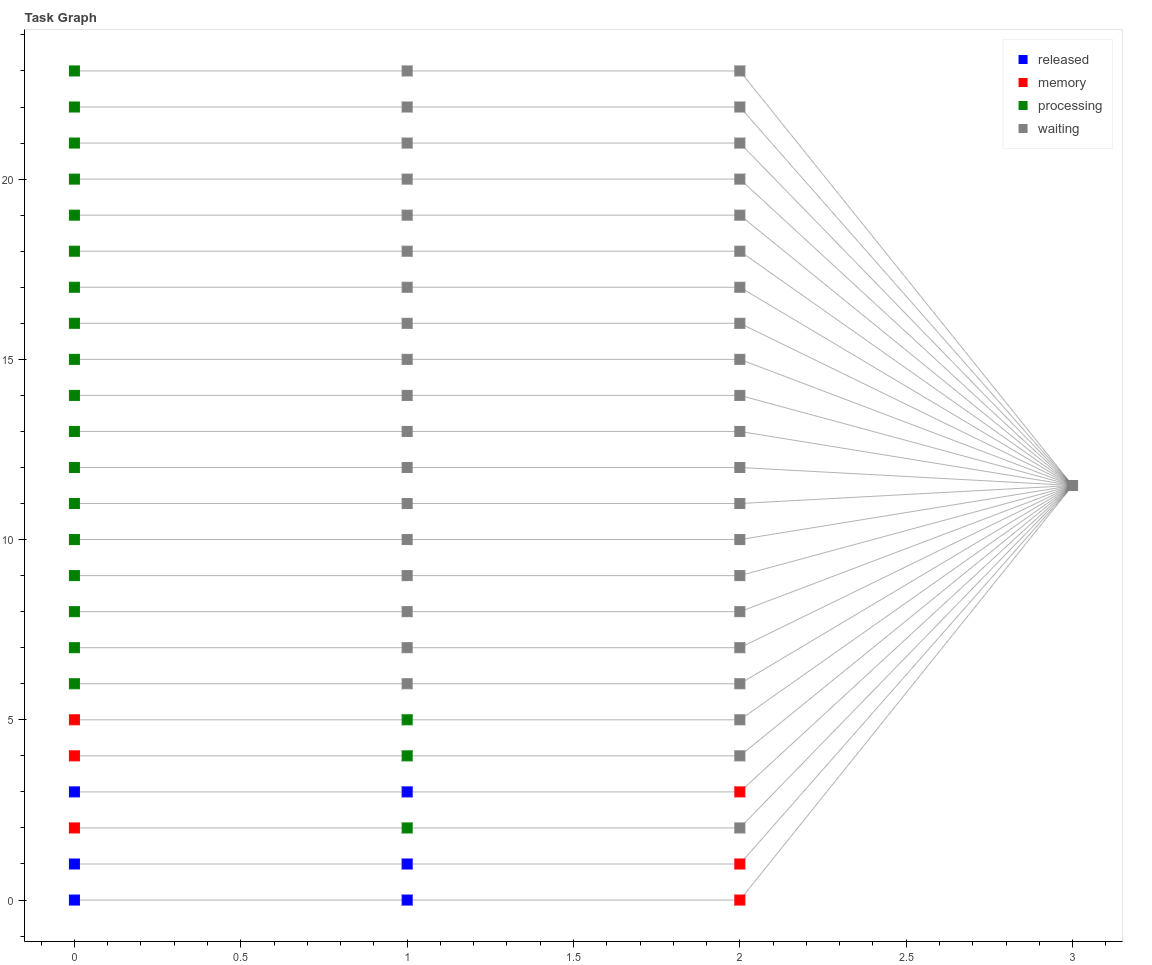
\includegraphics[width=0.7\linewidth]{task_plot.png}
  \end{figure} 
\end{frame}

\begin{frame}[t]{Simulation Framework}
  \begin{center}
  \textbf{Completely blind. You need to ask Tim.}
  \end{center}
  \\
  But here is what I know:
  \begin{itemize}
    \item Linear and non-linear effects present
    \item Currently only using chromosome 10
    \item $R^2$ between $0.04$ and $0.01$
  \end{itemize}
\end{frame}

\begin{frame}[t]{Some Results}
  \begin{figure}[htpb]
    \centering
    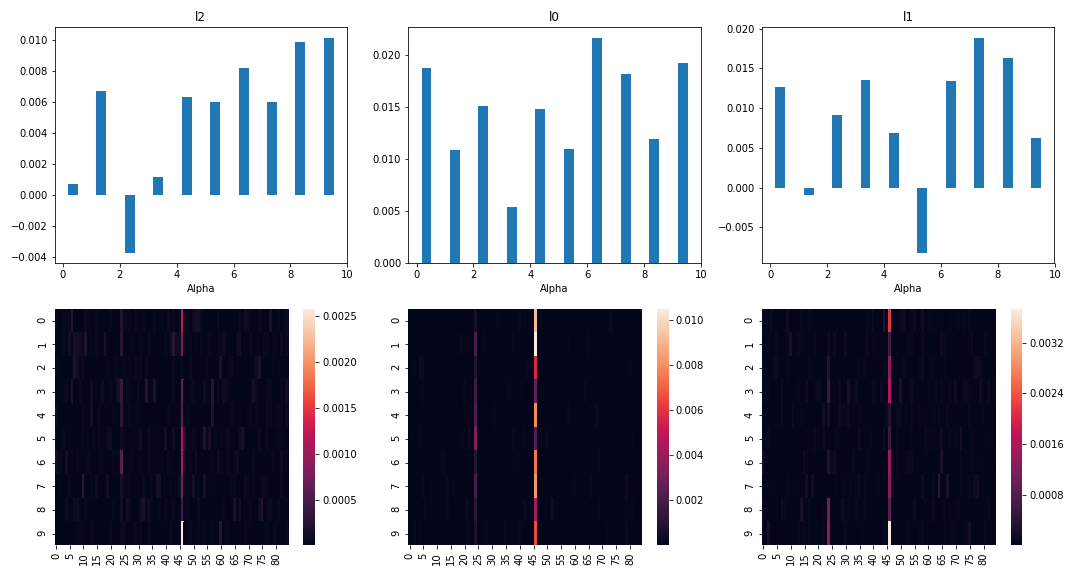
\includegraphics[width=0.99\linewidth]{performance.png}
    \caption{Performance}
  \end{figure}
\end{frame}

\begin{frame}[t]{Problem Assessment}
  \begin{figure}[htpb]
    \centering
    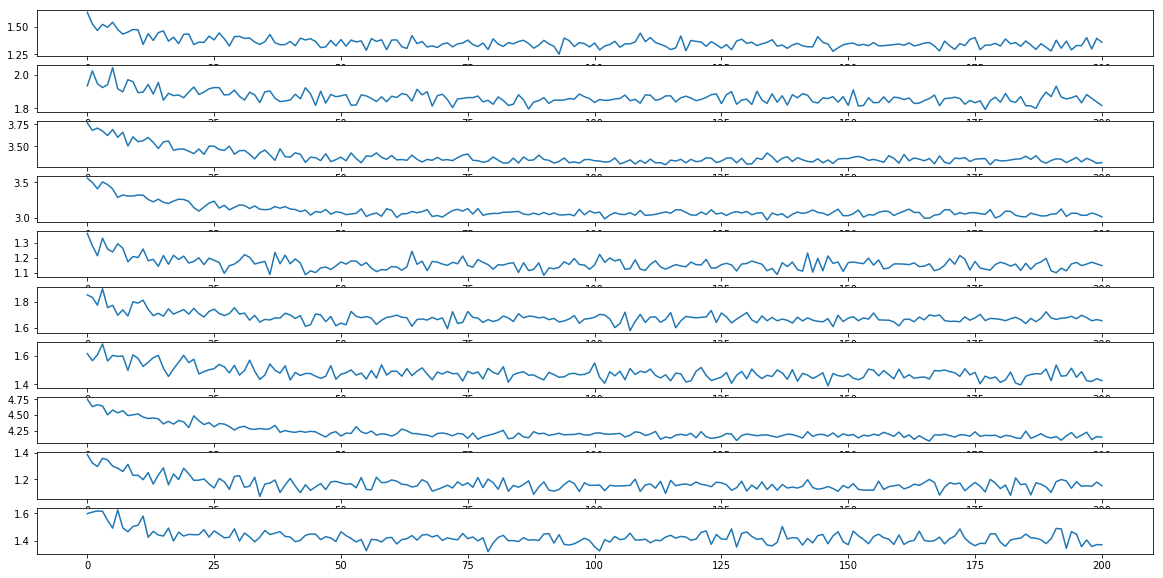
\includegraphics[width=0.8\linewidth]{loss_iteration_problem.png}
    \caption{Loss by iteration}
  \end{figure}
  \begin{itemize}
    \item mini-batch size too small ($n=500$)!
    \item number of iteration too small!
  \end{itemize}
\end{frame}

\begin{frame}[t]{Parameter Space}
  \begin{figure}[htpb]
    \centering
    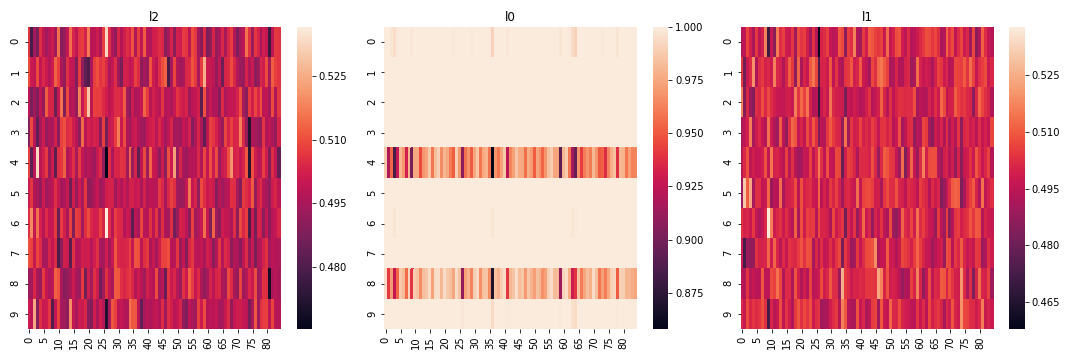
\includegraphics[width=0.99\linewidth]{null_proportion.png}
    \caption{Proportion of parameters equal or close to 0}
  \end{figure}
  \begin{itemize}
    \item $L_0$ comes very quickly to sparse solution (parameters are not accurate, small effects)
    \item $L_1$ and $L_2$ seem to take a bit longer
  \end{itemize}
\end{frame}
\end{document}
